\chapter{Resultados e Discussão}

Este capítulo visa apresentar os resultados obtidos durante a execução do projeto. O objetivo geral está presente na Seção \ref{sec:objetivos}, os objetivos específicos estão presentes na Seção \ref{sec:objetivos-especificos}, a metodologia utilizada está presente na Seção \ref{sec:metodologia}.

Em suma, o projeto tem por objetivo a criação de um pacote capaz de auxiliar desenvolvedores de aplicativos móveis utilizando o framework Flutter em criar aplicações mais acessíveis. Para isso, foi desenvolvido \texttt{linter} capaz de analisar o código-fonte de uma aplicação Flutter e identificar possíveis problemas de acessibilidade. O \texttt{linter} foi desenvolvido utilizando a linguagem de programação Dart e o pacote \href{https://pub.dev/packages/custom_lint_builder}{custom\_lint\_builder}.

O mesmo, já está publicado no repositório do \href{https://pub.dev/packages/accessibility_lint}{pub.dev} e pode ser utilizado por qualquer desenvolvedor Flutter que busca criar aplicações mais acessíveis. Na figura \ref{fig:pacote-publicado-pub-dev} é possível visualizar o mesmo, publicado.

\begin{figure}[!ht]
	\centering
	\caption{Pacote \href{https://pub.dev/packages/accessibility_lint}{accessibility\_lint} publicado no \href{https://pub.dev}{pub.dev}}\label{fig:pacote-publicado-pub-dev}
	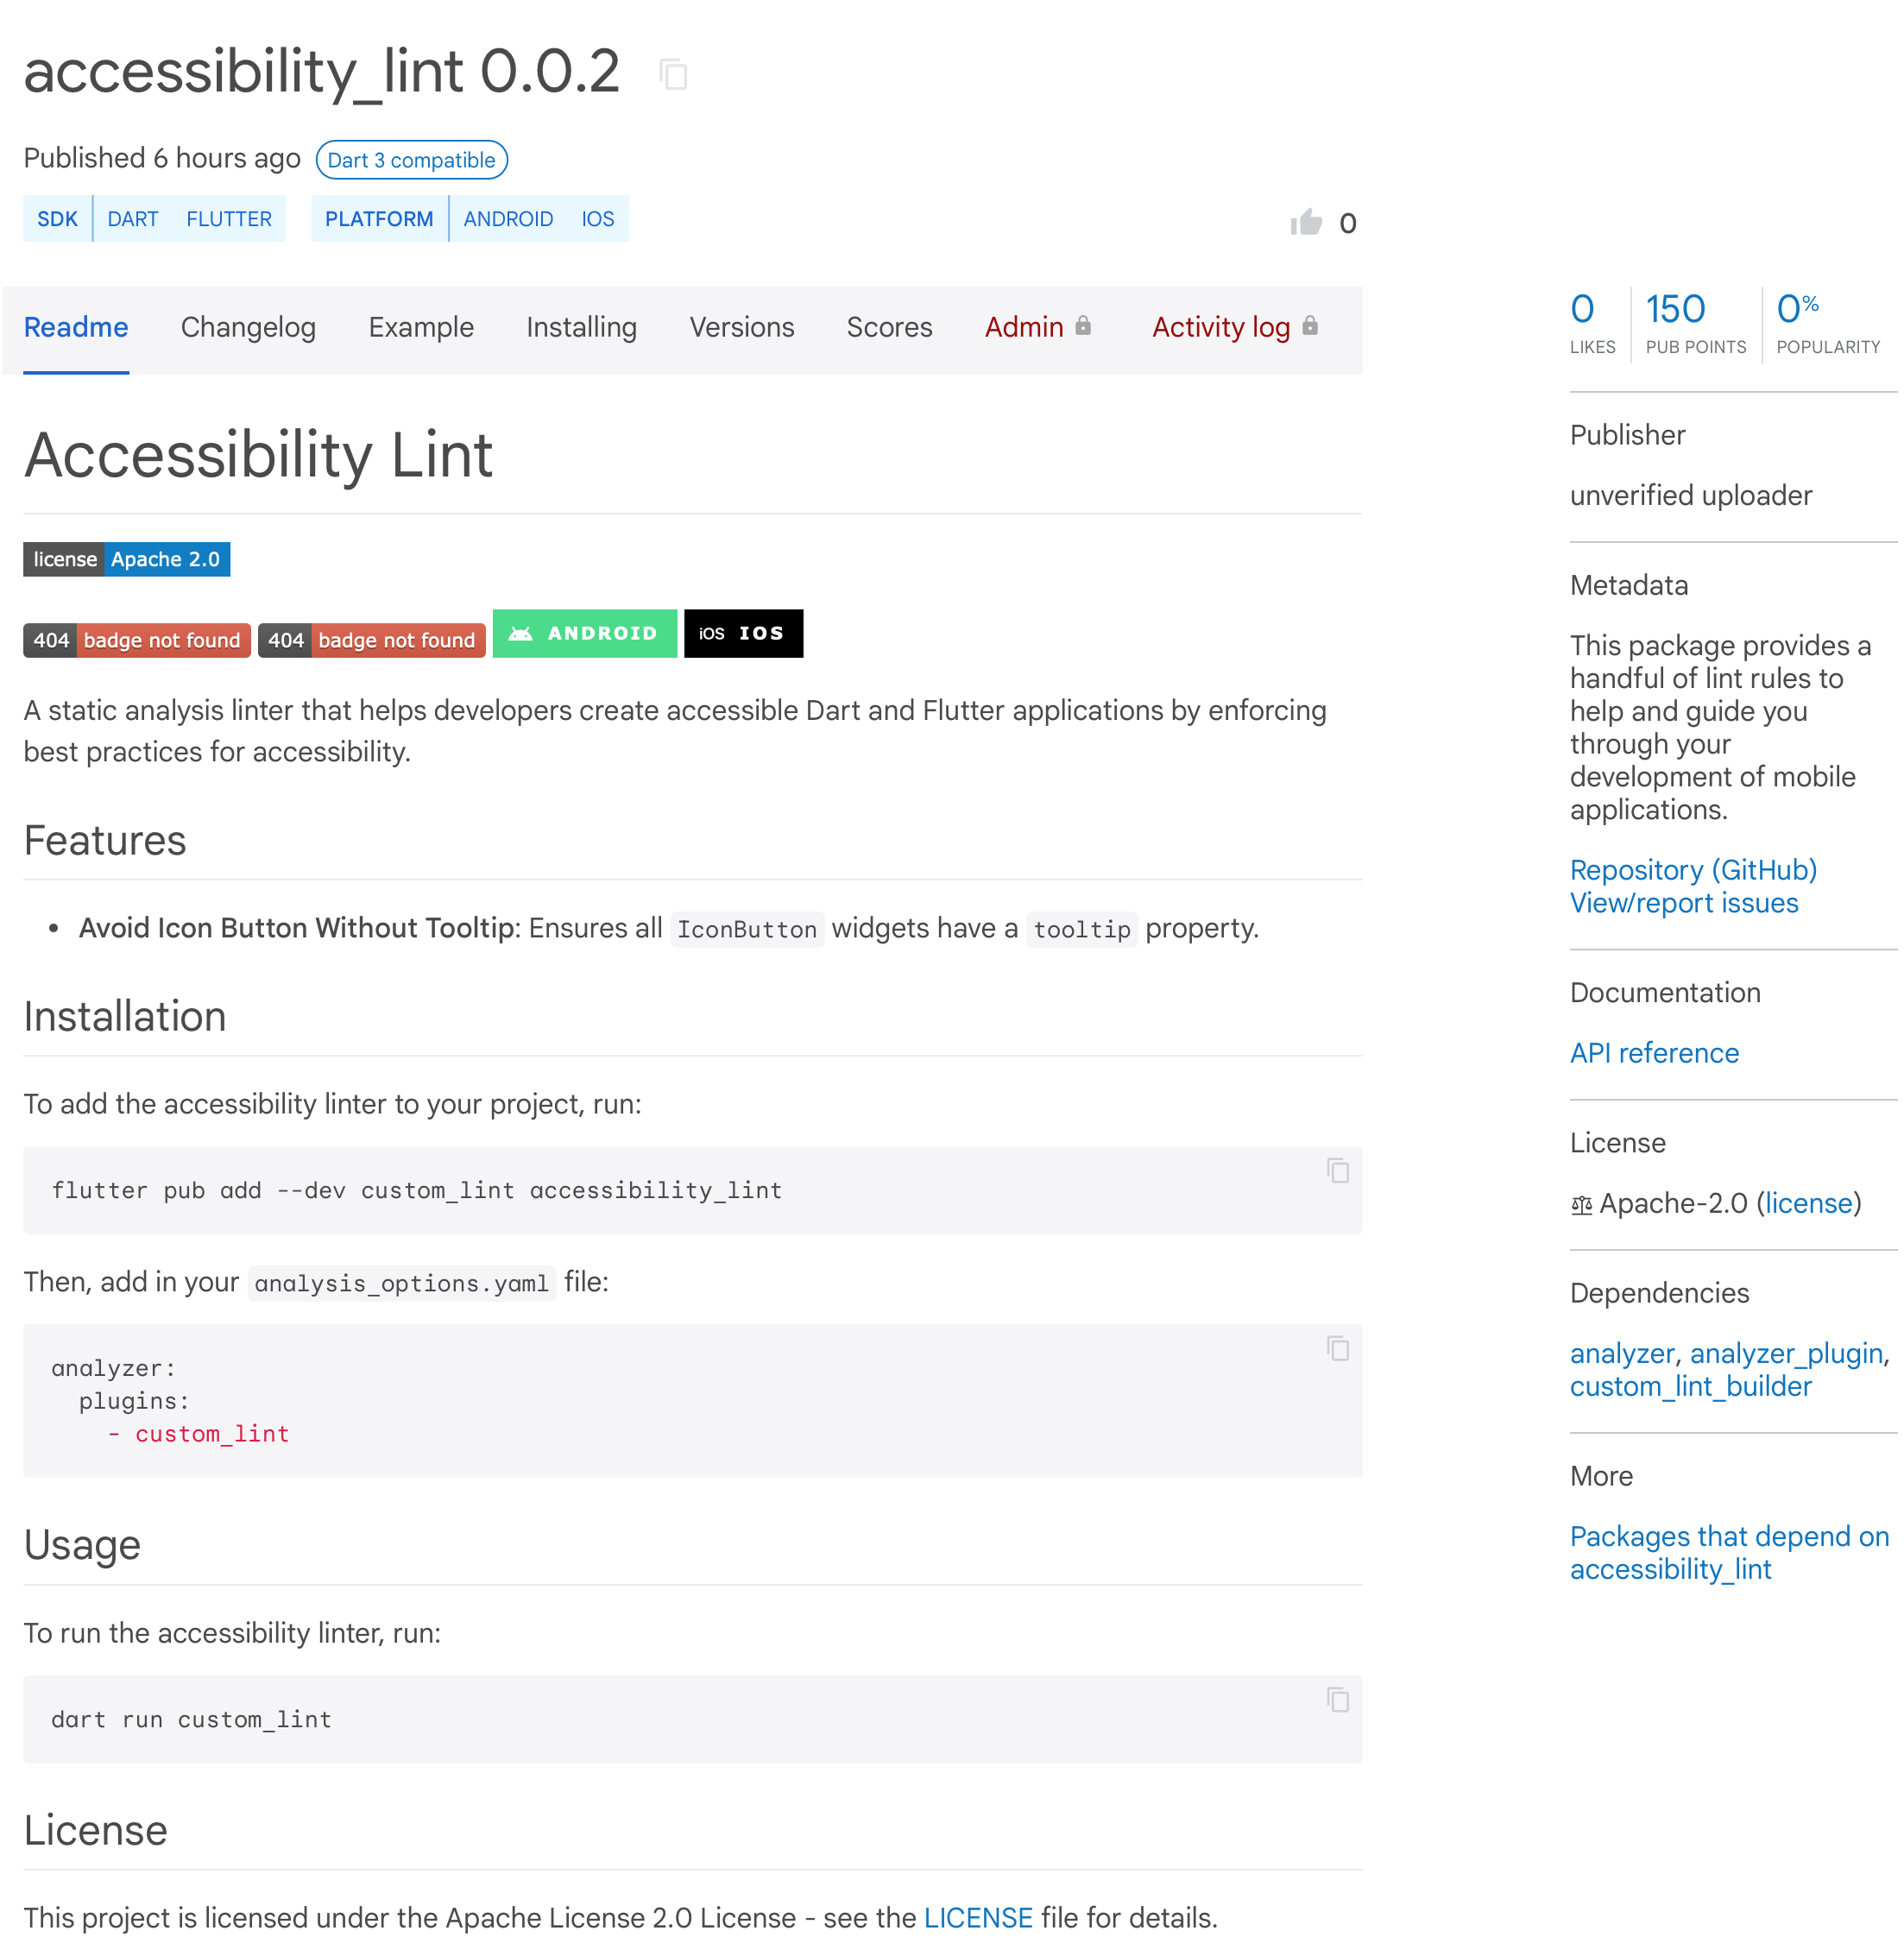
\includegraphics[width=400pt]{Assets/PacotePublicadoPubDev.png}
	\fonte{\me{2024}}
\end{figure}

A apresentação de sugestões de correção para os problemas identificados pelo \texttt{linter} é feita diretamente na sua IDE de desenvolvimento, através de mensagens de erro e avisos. A Figura \ref{fig:exemplo-codigo-fonte-tooltip} apresenta um exemplo de mensagem de erro gerada pelo \texttt{linter}.

\section{Objetivos e Requisitos}

O Objetivo Geral disposto na seção \ref{sec:objetivos} foi alcançado, uma vez que o pacote \seqsplit{accessibility\_lint} foi desenvolvido e publicado no repositório do \href{https://pub.dev/packages/accessibility_lint}{pub.dev} e pode ser utilizado por qualquer desenvolvedor Flutter que busca criar aplicações mais acessíveis.

Referente aos objetivos específicos dispostos na seção \ref{sec:objetivos-especificos}, o primeiro objetivo específico \ref{sec:revisao-literatura} foi alcançado, através do Mapeamento Sistemático da Literatura descrito na seção \ref{sec:msl}. Entretanto não chegou-se no objetivo esperado de construir uma relação de requisitos de acessibilidade para as plataformas Android e iOS. Para contornar, através da documentação de ambas as plataformas \cite{iosaccessibility}, \cite{androidaccessibility}, foi possível levantar alguns requisitos de acessibilidade dispostos na seção \ref{sec:regras-acessibilidade} como Regras de Acessibilidade. O segundo objetivo específico \ref{sec:projeto-implementacao} foi concluído com a implementação conforme disposta no capítulo \ref{sec:desenvolvimento}. E o terceiro objetivo específico \ref{sec:documentar-disseminar} teve seu objetivo alcançado uma vez que com o pacote publicado, e toda a pesquisa realizada, o conhecimento foi disseminado.

Agora será feita uma revisão dos Requisitos Funcionais (seção \ref{sec:requisitos-funcionais}), Requisitos não Funcionais (seção \ref{sec:requisitos-nao-funcionais}) e Regras de Negócio (seção \ref{sec:regras-negocio}).

A tabela \ref{tab:compara-requisitos} relaciona os requisitos funcionais implementados no desenvolvimento. Nela é possível verificar que quase todos os Requisitos Funcionais propostos foram implementados, com exceção do requisito \ref{req:consultar-requisitos} que não foi implementado. O mesmo se deu por conta da dificuldade em encontrar uma fonte confiável de Requisitos de Acessibilidade para as plataformas Android e iOS conforme disposto na seção \ref{sec:msl}.

\begin{table}[!htbp]
	\centering
	\renewcommand{\arraystretch}{1.1}
	\caption{Relação dos Requisitos implementados}
	\label{tab:compara-requisitos}
	\begin{tabular}{ L{11cm}  L{3cm} }
		\hline
    \textbf{Requisito} & \textbf{Implementado} \\
		\hline
    \ref{req:visualizar-inconsistencia} - O sistema deve permitir a visualização de inconsistências no código & \checkmark \\
    \ref{req:marcar-inconsistencia} - O sistema deve realizar marcações no código baseado na especificação definida & \checkmark \\
    \ref{req:sugerir-remover-inconsistencia} - O sistema deve sugerir remover trechos de código baseado na especificação definida & \checkmark \\
    \ref{req:sugerir-correcao-automatica} - O sistema deve sugerir correções automáticas baseado na especificação definida & \checkmark \\
    \ref{req:consultar-requisitos} - O sistema deve permitir o usuário consultar todos os requisitos não funcionais de acessibilidade & \ding{55} \\
    \ref{req:desabilitar-requisitos} - O sistema deve permitir o usuário desabilitar requisitos não funcionais de acessibilidade & \checkmark \\
    \ref{req:linha-comando} - O sistema deve permitir a utilização em ambientes de integração contínua & \checkmark \\
		\hline
  \end{tabular}
	\vspace{2mm}
	\fonte{\me{2024}}
\end{table}

A tabela \ref{tab:compara-requisitos-nao-funcionais} relaciona os requisitos não funcionais implementados no desenvolvimento. Nela é possível verificar que todos os Requisitos não Funcionais propostos foram implementados. Destaca-se que o pacote foi publicado no repositório do \href{https://pub.dev/packages/accessibility_lint}{pub.dev} e segue as melhores práticas para pacotes publicados no repositório \href{https://pub.dev}{pub.dev}. Com isso, todo e qualquer desenvolvedor Flutter pode utilizar o pacote para criar aplicações mais acessíveis.

\begin{table}[!htbp]
	\centering
	\renewcommand{\arraystretch}{1.1}
	\caption{Relação dos Requisitos não Funcionais implementados}
	\label{tab:compara-requisitos-nao-funcionais}
	\begin{tabular}{ L{11cm}  L{3cm} }
		\hline
    \textbf{Requisito não Funcional} & \textbf{Implementado} \\
		\hline
    \ref{rnf:utiliza-dart} - O sistema deve ser escrito utilizando a linguagem Dart & \checkmark \\
    \ref{rnf:pub-dev} - O sistema deve ser publicado no repositório \href{https:\\pub.dev}{pub.dev} & \checkmark \\
    \ref{rnf:melhores-praticas} - O sistema deve seguir as melhores práticas para pacotes publicados no repositório \href{https:\\pub.dev}{pub.dev} & \checkmark \\
    \ref{rnf:licenca-aberta} - O sistema deve possuir licença aberta para permitir alterações e melhorias & \checkmark \\
    \ref{rnf:documentacao} - O sistema deve possuir documentação para auxiliar na criação de novas regras de negócio de usabilidade & \checkmark \\
		\hline
  \end{tabular}
	\vspace{2mm}
	\fonte{\me{2024}}
\end{table}

\section{Regras de Acessibilidade}

Tendo em vista a não execução do Requisito Funcional \ref{req:consultar-requisitos}, não foi possível construir uma relação de Requisitos de Acessibilidade para as plataformas Android e iOS. Entretanto, foi possível levantar algumas Regras de Acessibilidade para o desenvolvimento do pacote \seqsplit{accessibility\_lint}. Os mesmos estão dispostos na tabela \ref{tab:regras-acessibilidade} e para facilitar visualização da implementação, a tabela \ref{tab:regras-acessibilidade-impl} relaciona as Regras de Acessibilidade com as implementações realizadas.

\begin{table}[!htbp]
	\centering
	\renewcommand{\arraystretch}{1.1}
	\caption{Relação das Regras de Acessibilidade implementadas}
	\label{tab:regras-acessibilidade-impl}
	\begin{tabular}{ L{11cm}  L{3cm} }
		\hline
    \textbf{Regra de Acessibilidade} & \textbf{Implementado} \\
		\hline
    \ref{ra:tooltip} - Utilize rótulos descritivos para todos os elementos interativos & \checkmark \\
    \ref{ra:descricao-imagens} - Forneça descrições de texto alternativas para imagens & \checkmark \\
    \ref{ra:feedback-visual} - Forneça feedback visual, auditivo ou tátil para todas as interações do usuário & \checkmark \\
    \ref{ra:largura-minima} - Elementos interativos devem possuir um mínimo de 48pt de largura e altura & \checkmark \\
    \ref{ra:contraste-minimo} - Forneça um contraste mínimo de 4.5:1 entre o texto e o plano de fundo & \ding{55} \\
		\hline
  \end{tabular}
	\vspace{2mm}
	\fonte{\me{2024}}
\end{table}

A regra de acessibilidade \ref{ra:contraste-minimo} não foi implementada por conta da dificuldade em encontrar uma forma de verificar o contraste entre o texto e o plano de fundo. Uma vez que elementos podem utilizar diferentes fontes para sua cor de fundo e ou texto.

Ao final, temos como resultado a implementação de 4 Regras de Acessibilidade dispostas em diferentes implementações ao longo do projeto, uma vez que as mesmas foram sub dividas para atender melhor a Regrar. Por exemplo, a regra de acessibilidade \ref{ra:tooltip} foi implementada através da criação de regras para Botões com \texttt{IconButton} e \texttt{ElevatedButton}, \texttt{TextButton}, \texttt{OutlinedButton} e \texttt{FloatingActionButton}, \texttt{Radio}, \texttt{Switch} e outros elementos interativos.
